\documentclass[border=3pt]{standalone}

% Drawing
\usepackage{tikz}

%Notation
\usepackage{amsmath}

% Tikz Library 
\usetikzlibrary{angles, quotes, shapes, decorations.markings, calc, arrows.meta}

% Styles
%% Node Style in Order Text to Get Center Alignment
\tikzset{every text node part/.style={align=center}}
%% Main Ray Style
\tikzset{ray/.style = {postaction=decorate,decoration={markings,
						 mark=at position .49 with \arrow{stealth},
						 mark=between positions 0.1 and 0.4 step 0.5cm with with{
						 \draw[fill=red, draw = red] circle[radius=1pt];
						 \draw[red, {Latex[length=1.3mm, width=1.5mm]}-{Latex[length=1.3mm, width=1.5mm]}] (0,-7pt) -- (0,7pt);},
						 mark=between positions 0.6 and 0.9 step 0.5cm with with{
						 \draw[fill=red, draw = red] circle[radius=1pt];
						 \draw[red, {Latex[length=1.3mm, width=1.5mm]}-{Latex[length=1.3mm, width=1.5mm]}] (0,-7pt) -- (0,7pt);}
						 								}
						 }
		}	
%% Bottom Ray Inside Box
\tikzset{rayE1/.style = {postaction=decorate,decoration={markings,
						 mark=at position .52 with \arrow{stealth},
						 mark=between positions 0.65 and 0.9 step 0.7cm with with{
						 \draw[red, {Latex[length=1.3mm, width=1.5mm]}-{Latex[length=1.3mm, width=1.5mm]}] (0,-7pt) -- (0,7pt);
						 \draw[fill=black!10, draw = black!10] circle[radius=1pt];}
						 								}
						 }
		}
%% Bottom Ray Outside Box
\tikzset{rayE2/.style = {postaction=decorate,decoration={markings,
						 mark=at position .52 with \arrow{stealth},
						 mark=between positions 0.1 and 0.4 step 0.54cm with with{
						 \draw[red, {Latex[length=1.3mm, width=1.5mm]}-{Latex[length=1.3mm, width=1.5mm]}] (0,-7pt) -- (0,7pt);
						 \draw[fill=white, draw = white] circle[radius=1pt];},
						 mark=between positions 0.6 and 0.9 step 0.5cm with with{
						 \draw[red, {Latex[length=1.3mm, width=1.5mm]}-{Latex[length=1.3mm, width=1.5mm]}] (0,-7pt) -- (0,7pt);
						 \draw[fill=white, draw = white] circle[radius=1pt];}
						 								}
						 }
		}
%% Upper Ray Inside Box
\tikzset{rayT1/.style = {postaction=decorate,decoration={markings,
						 mark=at position .52 with \arrow{stealth},
						 mark=between positions 0.65 and 0.9 step 0.7cm with with{
						 \draw[fill=red, draw = red] circle[radius=1pt];}
						 								}
						 }
		}
%% Upper Ray Outside Box		
\tikzset{rayT2/.style = {postaction=decorate,decoration={markings,
						 mark=at position .52 with \arrow{stealth},
						 mark=between positions 0.1 and 0.4 step 0.54cm with with{
						 \draw[fill=red, draw = red] circle[radius=1pt];},
						 mark=between positions 0.6 and 0.9 step 0.5cm with with{
						 \draw[fill=red, draw = red] circle[radius=1pt];}
						 								}
						 }
		}

\begin{document}

	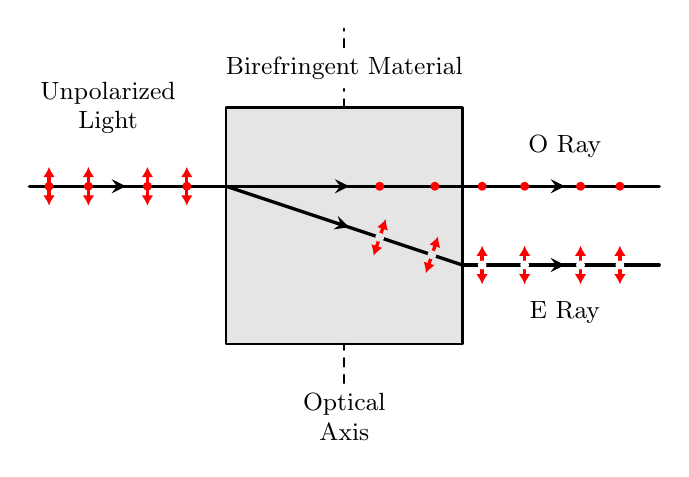
\begin{tikzpicture}[line cap=round, line join=round]
		% Grid
%		\draw[dotted, black!20] (0,0) grid (8,8);
%		
%		\node at (-2ex,-2ex) {$0$};
%		\foreach \i in {1,...,8}
%		{
%			\node at (-2ex,\i) {$\i$};
%			\node at (\i,-2ex) {$\i$};
%		}
		
		% Coordinates
		\coordinate (A) at (0,2);
		\coordinate (B) at (2.5,2);
		%
		\coordinate (B') at (5.5,2);
		\coordinate (B'') at (5.5,1);
		\coordinate (C') at (8,2);
		\coordinate (C'') at (8,1);
		
		%Rectangle
		\draw[thick, fill=black!10] (2.5,0) rectangle (5.5,3);	
		
		% Rays
		\draw[very thick, ray] (A) -- (B);
		%% Upper Ray
		\draw[very thick, rayT1] (B) -- (B');	
		\draw[very thick, rayE1] (B) -- (B'');	
		%% Bottom Ray
		\draw[very thick, rayT2] (B') -- (C');
		\draw[very thick, rayE2] (B'') -- (C'');

		% Nodes
		\node at (1,3) {\small Unpolarized\\[-0.5mm]\small Light};
		\node at (6.8,2.5) {\small $\mathrm{O}$ Ray};
		\node at (6.8,0.4) {\small $\mathrm{E}$ Ray};
		\node at (4,3.5) (node) {\small Birefringent Material};
		
		% Dashed Axis
		\draw[dashed, thick] (4,-0.5) -- (4,0) node[pos=0, below] {\small{Optical}\\[-0.5mm]\small{Axis}};
		\draw[dashed, thick] (4,3) -- (node) -- (4,4);
	\end{tikzpicture}
	
\end{document}
